\documentclass[10pt]{beamer}

% Configuration {{{
\usepackage[utf8]{inputenc}
\usepackage[T2A]{fontenc} % T1 for English
\usepackage[english, russian]{babel}

\usepackage{mathtools}
\usepackage{graphicx}
\usepackage[multidot]{grffile}
\usepackage[labelsep=period]{caption}

\setbeamertemplate{caption}[numbered]
\setbeamertemplate{navigation symbols}{}
\usefonttheme[onlymath]{serif}
\usepackage{DejaVuSansCondensed} % helvet for English
\usetheme{Madrid}

\linespread{1.2}
\setlength{\parskip}{.3\baselineskip}

\def\what#1{\textcolor{lightgray}{#1}}
\def\meh#1{\textcolor{gray}{#1}}
% }}}

\title[ATLAS -- ANL (USA)]{Argonne Tandem Linac Accelerator System -- линейный ускоритель тяжелых ионов в~Argonne National Laboratory (USA)}
\author[Керим Гусейнов]{Керим Гусейнов}
\institute[]{МГУ им. М. В. Ломоносова}
\date{17 ноября 2021 г.}

\begin{document}

\frame[plain]{% Title page {{{
	\titlepage
}% }}}

\frame{% whole pic {{{
	% Ускорительный комплекс атлас схематически выглядит следующим 
	% образом.
	%
	% Три ускорительные секции: PII -- инжектор положительных ионов, 
	% бустер и сам atlas. Общее напряжение вплоть до 50 мега вольт, 
	% и ускоряться принципиально могут ядра от протона до урана.
	%
	% RFQ -- радиочастотный квадруполь
	%
	% ECR -- electron cyclotron resonance source of ions
	%
	% RIB -- radioactive ion beams
	% 
	% EBIS -- electron beam ion source
	% CARIBU -- Californium Rare Isotope Breeder Upgrade
	%
	% Кроме ускорителей, важной частью является caribu -- система, 
	% позволяющая выделять нейтроноизбыточные осколки спонтанного распада 
	% калифорния 252.
	%
	% Каждый год проводится примерно 50 экспериментов, занимающих около 
	% 6000 часов работы (8 мес в год).
	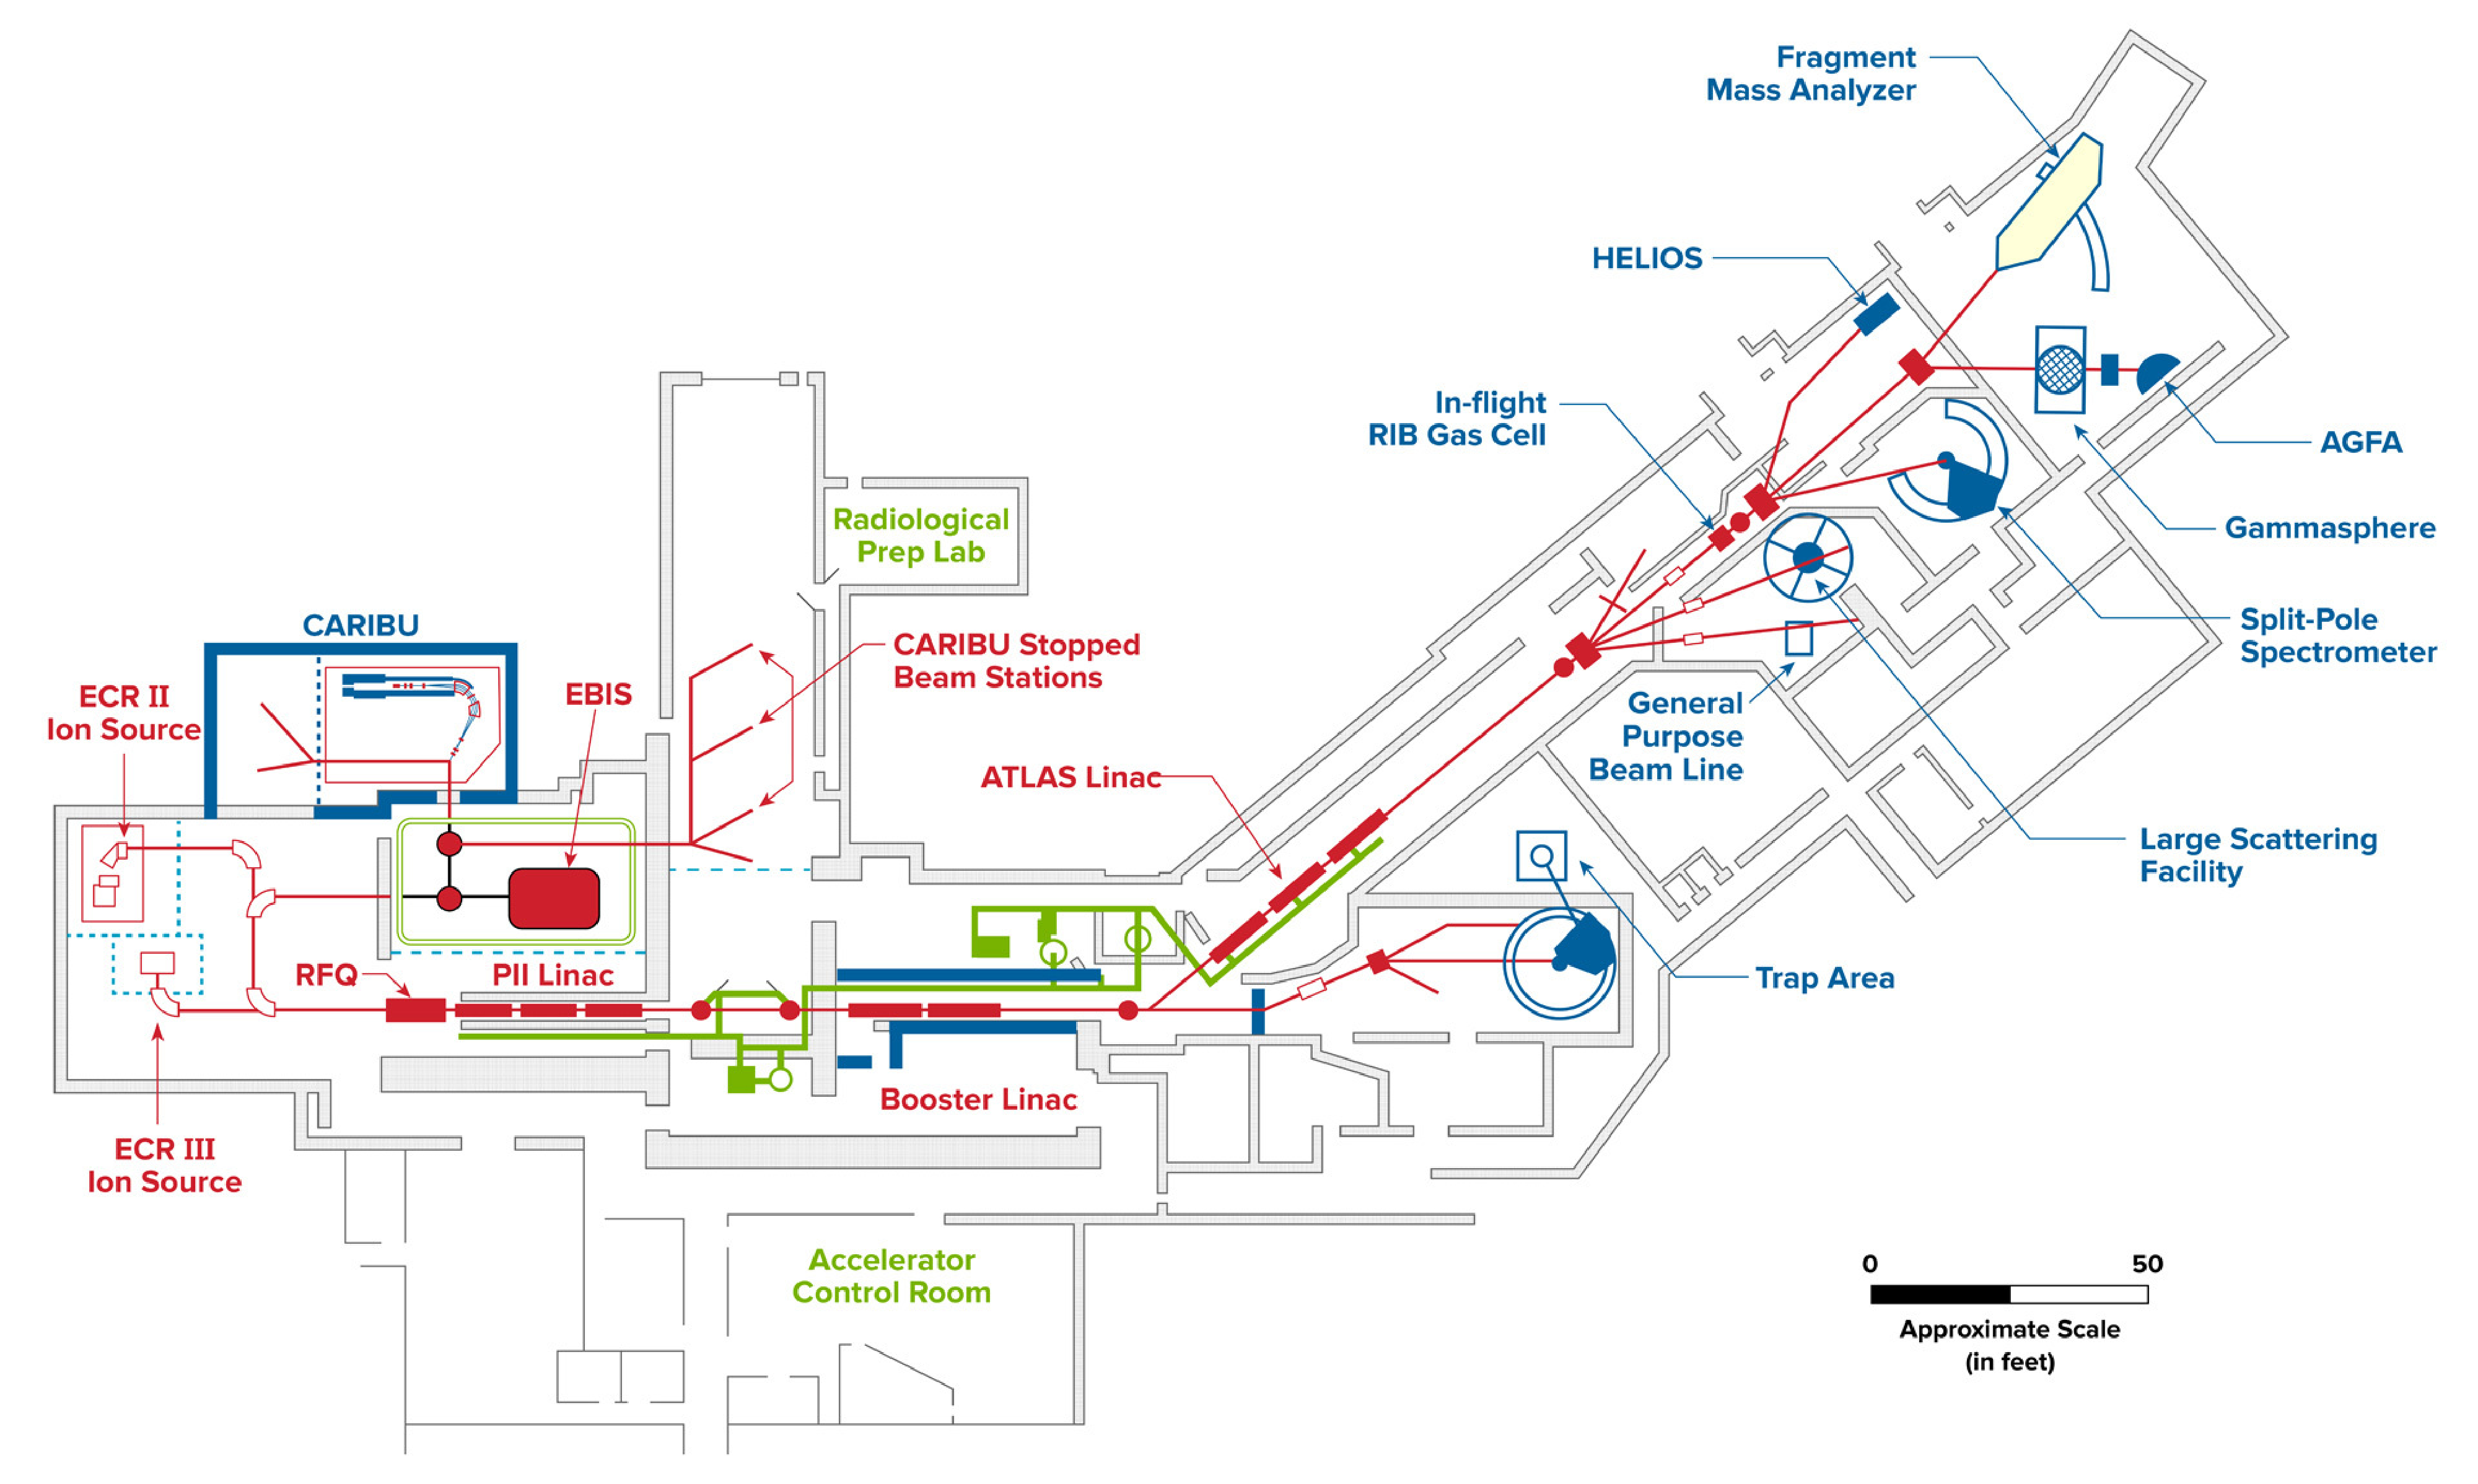
\includegraphics[width=\textwidth]{figures/floor-plan}
}% }}}
\frame{% whole pic text {{{
	Ускорительный комплекс атлас содержит три ускорительные секции: 
	инжектор положительных ионов (Positive Ion Injector), бустер и сам 
	atlas. Суммарное напряжение этих трех частей достигает 50 мегавольт, 
	и ускоряться принципиально могут любые ядра от протона до урана.

	RFQ -- радиочастотный квадруполь, предназначенный для фокусировки 
	пучка.

	ECR -- electron cyclotron resonance -- источник ионов, ионизатор.

	% RIB -- radioactive ion beams

	EBIS -- electron beam ion source

	CARIBU -- Californium Rare Isotope Breeder Upgrade

	Кроме ускорителей, важной частью комплекса является CARIBU -- система, 
	позволяющая выделять определенные нейтроноизбыточные осколки 
	спонтанного распада калифорния 252.
}% }}}

\frame{% in-flight {{{
	% Кроме того, система атлас предоставляет еще и пучки легких 
	% радиоактивных ядер вблизи долины стабильности. Для их получения 
	% пучок из ускорителя направляют в газовую камеру или на фольгу, где 
	% ядра пучка проходят через реакции нуклонного обмена, а затем 
	% продукты фокусируются и направляются уже в нужную мишень. Для 
	% повышения качества и чистоты пучка мгновенно распадающиеся обратно 
	% продукты отделяются, а также производится отбор по импульсу.
	%
	% Таким образом в роли налетающей частицы может выступать целый ряд 
	% радиоактивных легких ядер до массы около 40.
	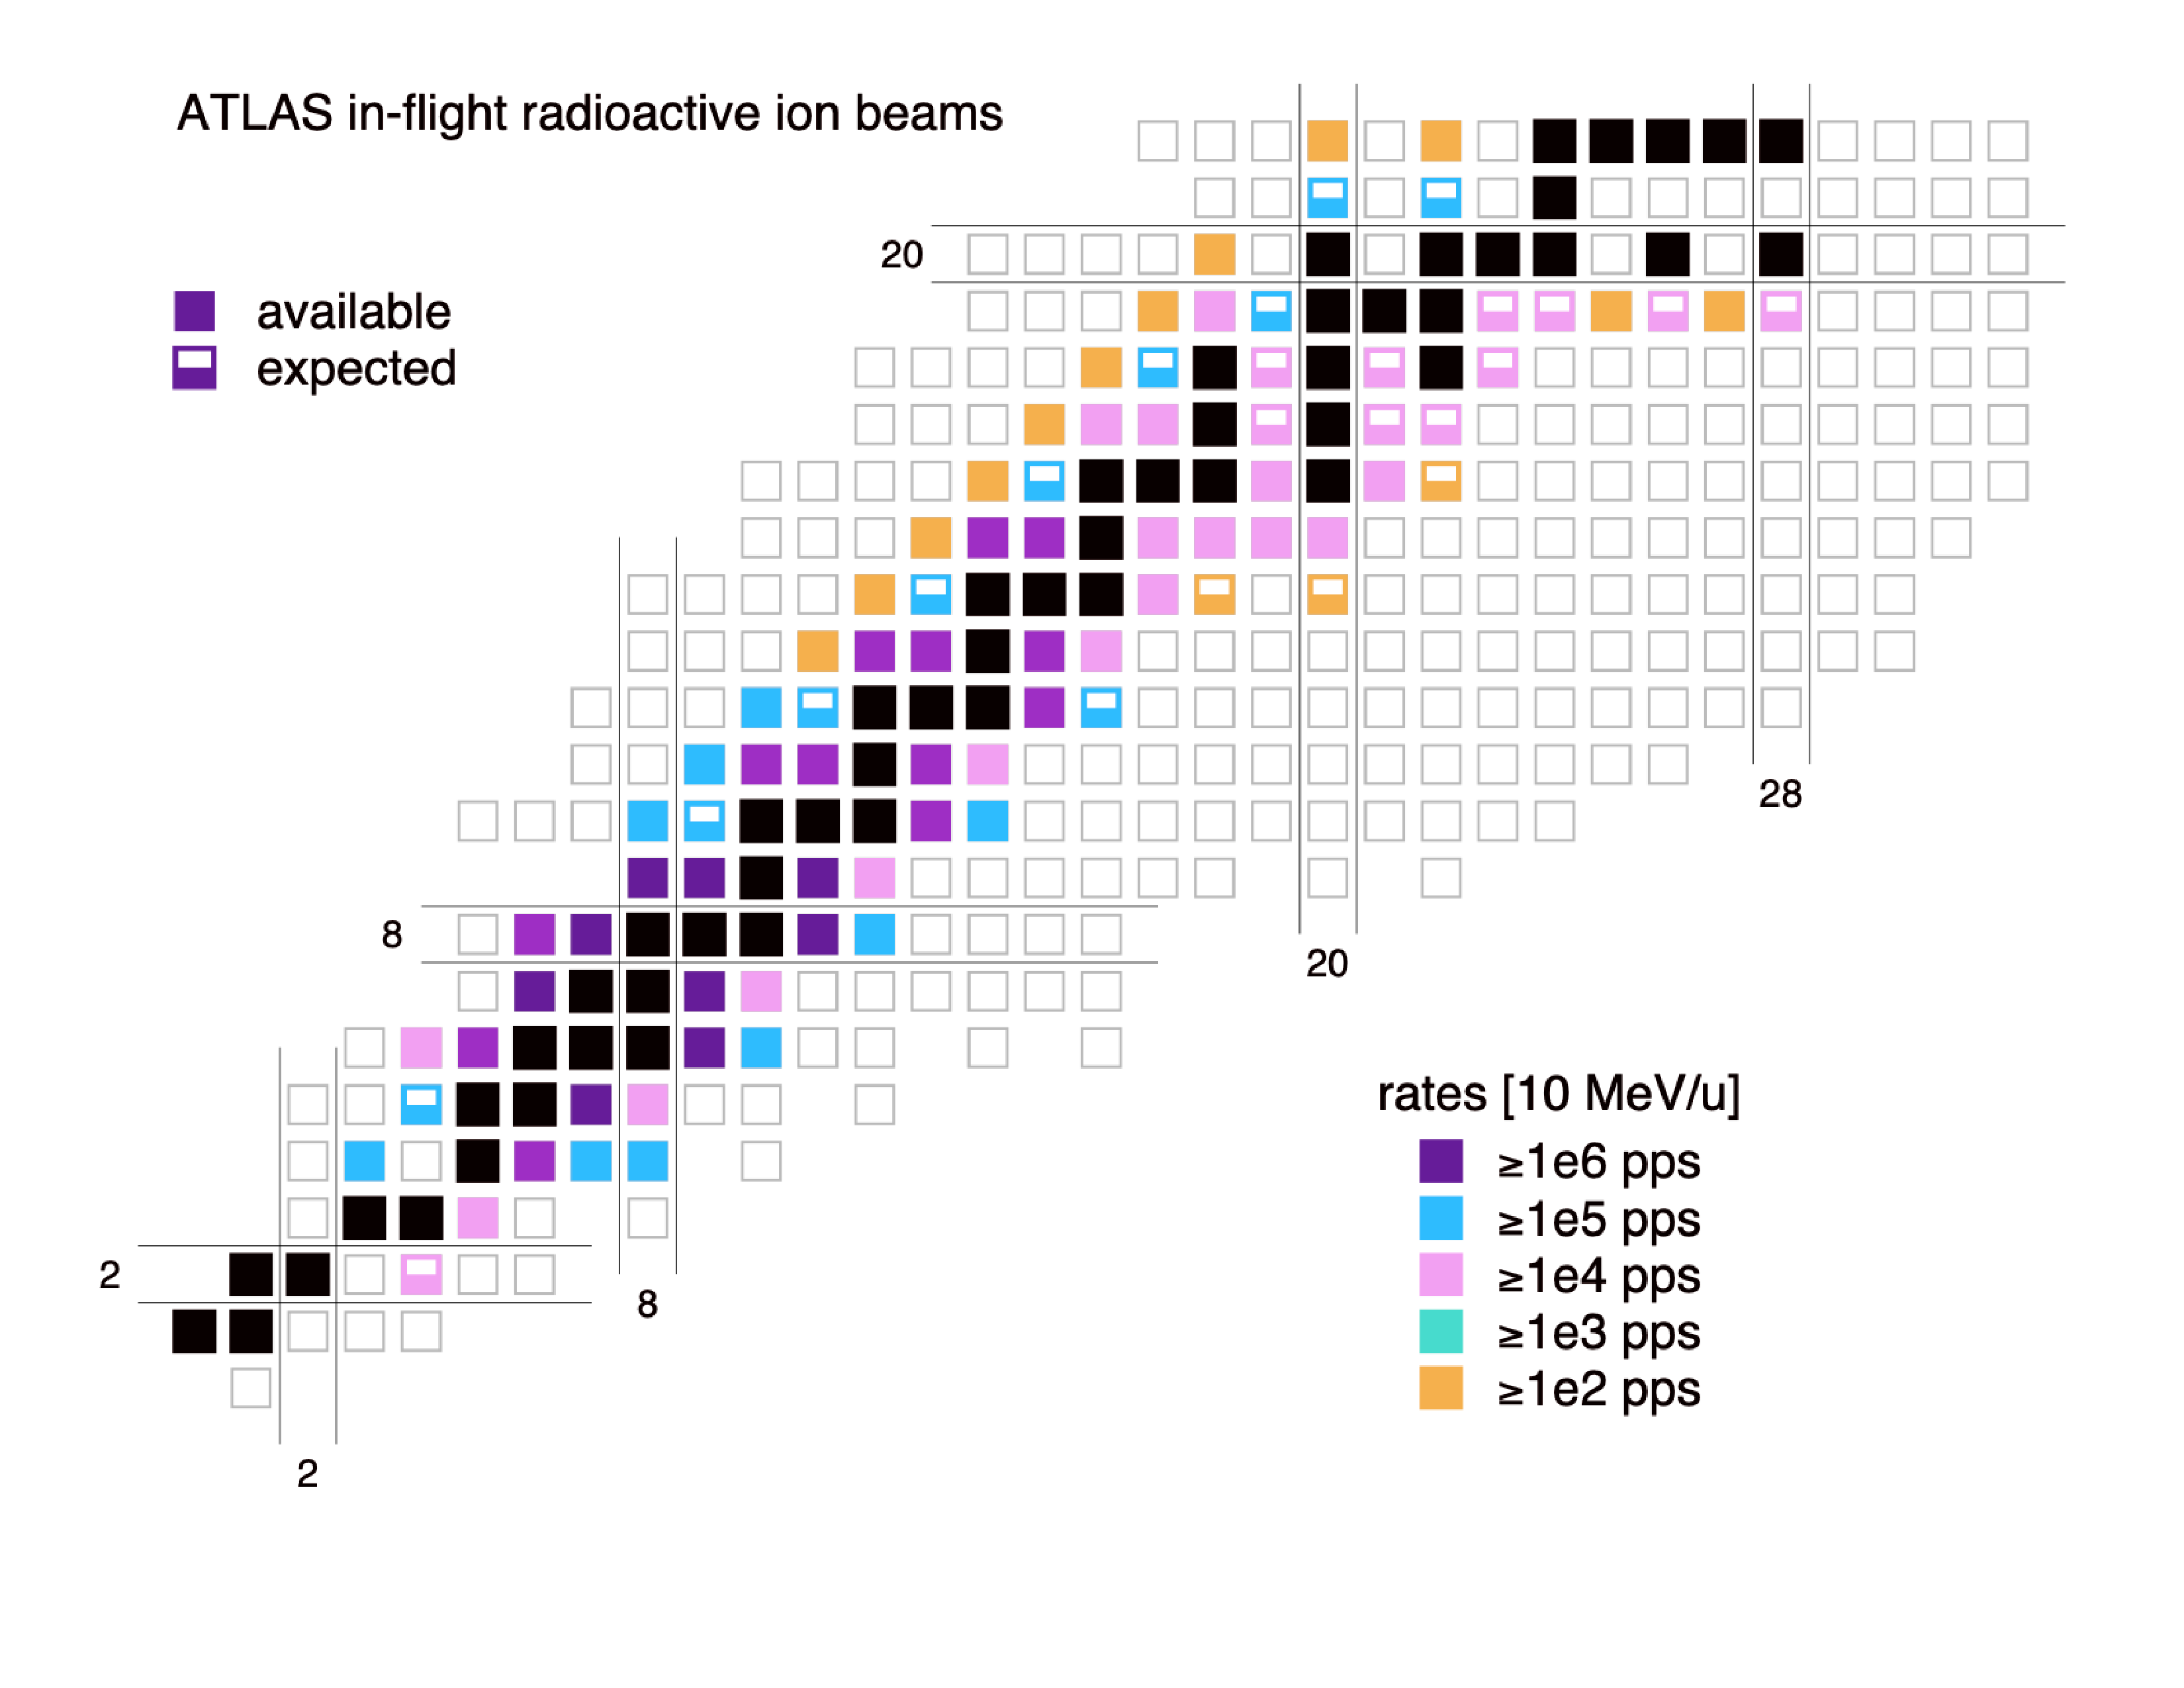
\includegraphics[width=\textwidth]{figures/in-flight-nuclei}
}% }}}
\frame{% in-flight text {{{
	Кроме того, система атлас предоставляет еще и пучки легких 
	радиоактивных ядер вблизи долины стабильности. Для их получения 
	пучок из ускорителя направляют в газовую камеру или на фольгу, где 
	ядра пучка проходят через реакции нуклонного обмена, а затем 
	продукты фокусируются и направляются уже в нужную мишень. Для 
	повышения качества и чистоты пучка мгновенно распадающиеся обратно 
	продукты отделяются, а также производится отбор по импульсу.

	Таким образом, в роли налетающей частицы может выступать целый ряд 
	радиоактивных легких ядер массами до примерно 40.
}% }}}

\frame{% neutron rich {{{
	\frametitle{CARIBU -- подача продуктов распада $^{252}$Cf}
	% калифорний распадается в камере с очень чистым гелием (газом), где 
	% фрагменты быстро теряют энергию, затем ускоряются до 30кЭв и масс 
	% анализируются, а затем переносятся к EBIS и к квадруполю RFQ 
	% в начало ускорительных дел.
	% Примерно половина продуктов становятся +1 или +2 ионами, а между 
	% распадом калифорния и квадруполем основным проходит около 40 мс. 
	% Кроме того разделение продуктов очевидно не зависит от химических 
	% свойств.
	%
	% Ускоряются они тут до 15 МэВ/нуклон
	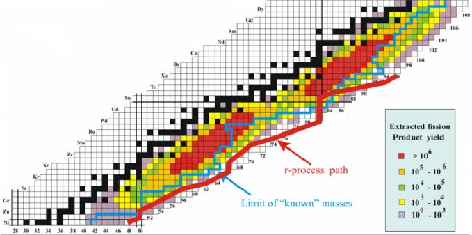
\includegraphics[width=\textwidth]{figures/cf-products}
}% }}}
\frame{% neutron rich text {{{
	\frametitle{CARIBU -- подача продуктов распада $^{252}$Cf}
	Калифорний распадается в камере с очень чистым гелием (газом), где 
	фрагменты быстро теряют энергию, затем ускоряются до 30~КэВ и попадают 
	в масс-анализатор, где производится отбор. Затем они переносятся 
	к EBIS и к квадруполю RFQ в начало самого ускорителя.

	Примерно половина продуктов становятся ионами с зарядом +1 или +2, 
	а между распадом калифорния и попаданием в квадруполи проходит около 
	40 мс. Кроме того разделение продуктов очевидно не зависит от
	химических свойств.

	Ускоряются такие ядра до 15 МэВ/нуклон

	Максимальные энергии стабильных ядер изменяются от 18-20~МэВ/нуклон 
	для легких до 9-10 для тяжелых.

	Нестабильные легкие достигают около 15 МэВ/нуклон вместо 20.
}% }}}

\frame{% pie chart for projectiles {{{
	% Максимальные энергии изменяются от 18-20 МэВ/нуклон для легких до 
	% 9-10 для тяжелых.
	%
	% Для легких нестабильных около 15 вместо 20.
	\centering
	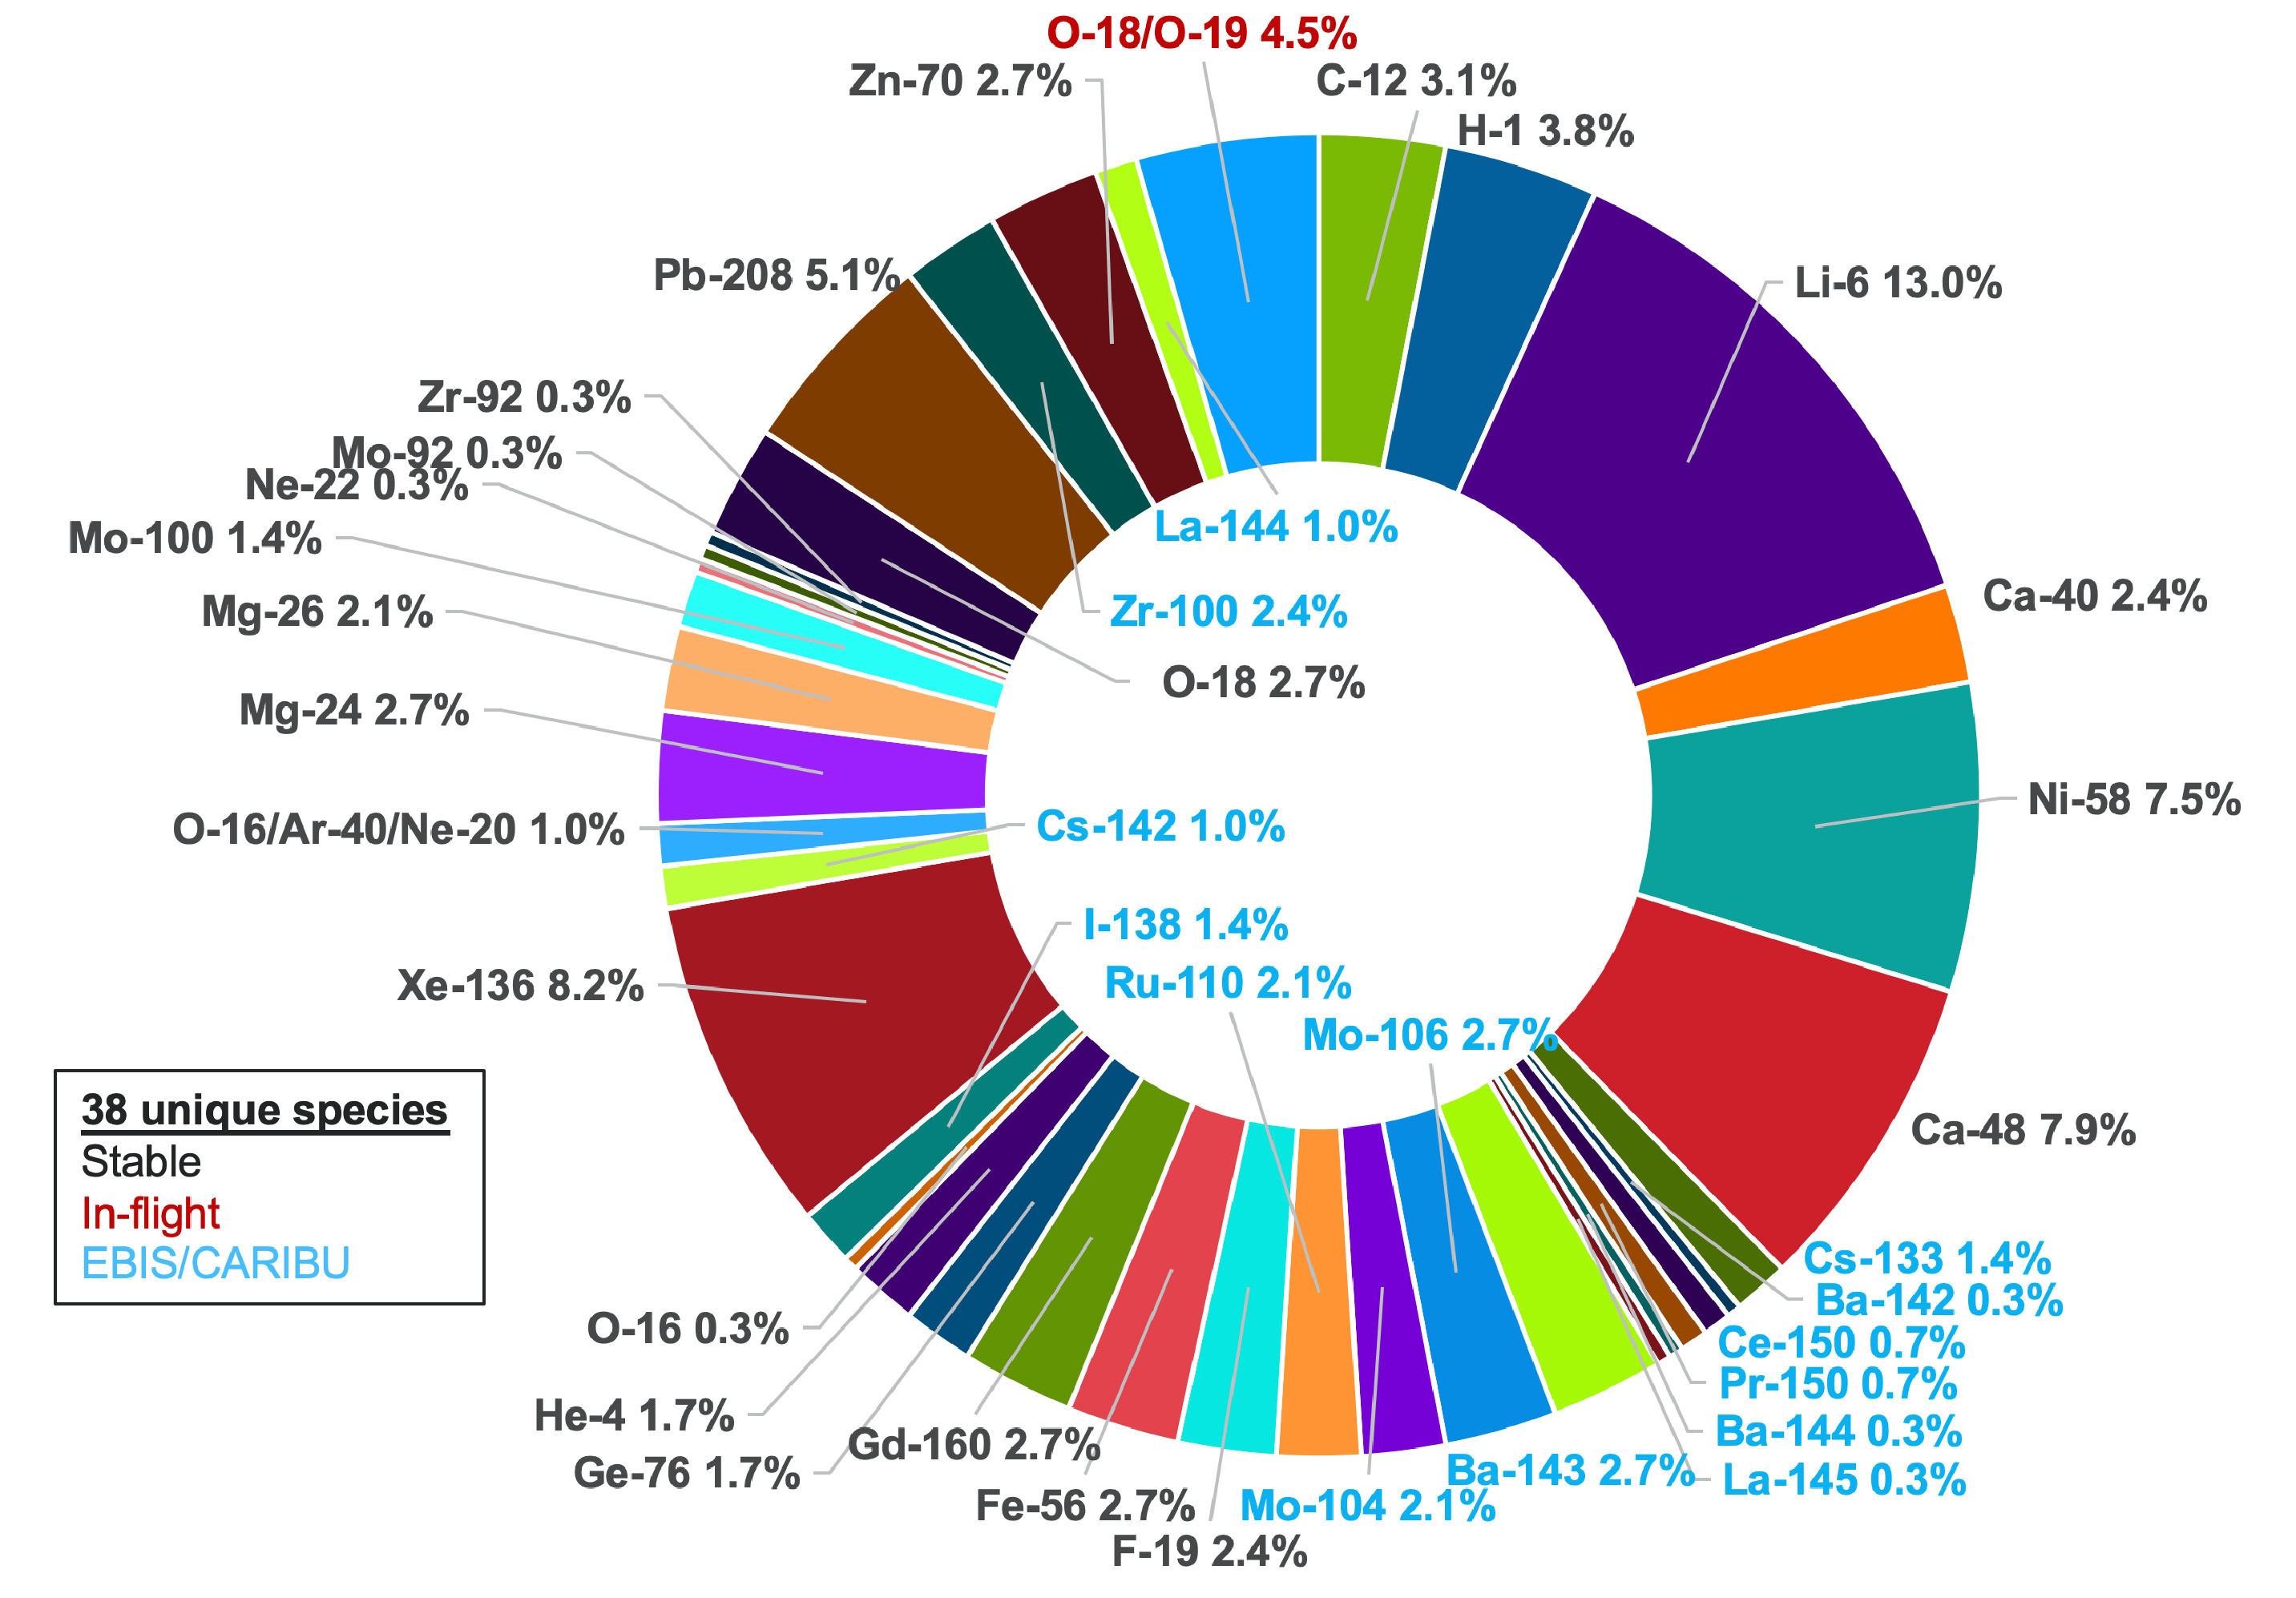
\includegraphics[width=.9\textwidth]{figures/stable}

	\small

	Выше показаны доли наиболее часто используемых ядер. Каждый год 
	проводится примерно 50 экспериментов, суммарно занимающих около 6000 
	часов работы (8 месяцев в год).
}% }}}

\frame{% whole pic for targets {{{
	% анализатор фрагментов масс используется для разделения продуктов 
	% реакции на интересующей мишени и непровзаимодействовавших ядер. 
	% Также он используется в схеме совпадений при одновременной 
	% регистрации фотонов и ядер. И еще позволяет разделять ядра с разными 
	% отношениями заряда к массе.
	%
	% HELIOS это винтовой орбитальный спектрометр, или спектрометр 
	% с винтовыми орбитами... Здесь мишень располагается прям внутри 
	% соленоида, который представляет собой напрямую магнит из МРТ. Мишень 
	% и детектор находятся на оси соленоида, а продукты реакции загибаются 
	% и летят обратно к оси. Детектор можно переставлять так, чтобы ловить 
	% продукты с определенной энергией, зарядом и прочее. На гелиосе 
	% изучают реакции передачи одного или нескольких нуклонов, кластеров, 
	% неупругое рассеяние, используют в основном для нестабильных пучков.
	%
	% AGFA -- argonne gas filled separator -- газовый сепаратор, 
	% используется для изучения тяжелых и сверхтяжелых ядер. Например, 
	% поиск изомерных состояний в таких ядрах и изучение ядер вблизи 
	% протонной радиоактивности. Изучение тяжелых нейтроноизбыточных ядер 
	% в глубоконеупругих реакциях...
	%
	% gammasphere состоит из 100 германиевых детекторов, детектор фотонов.
	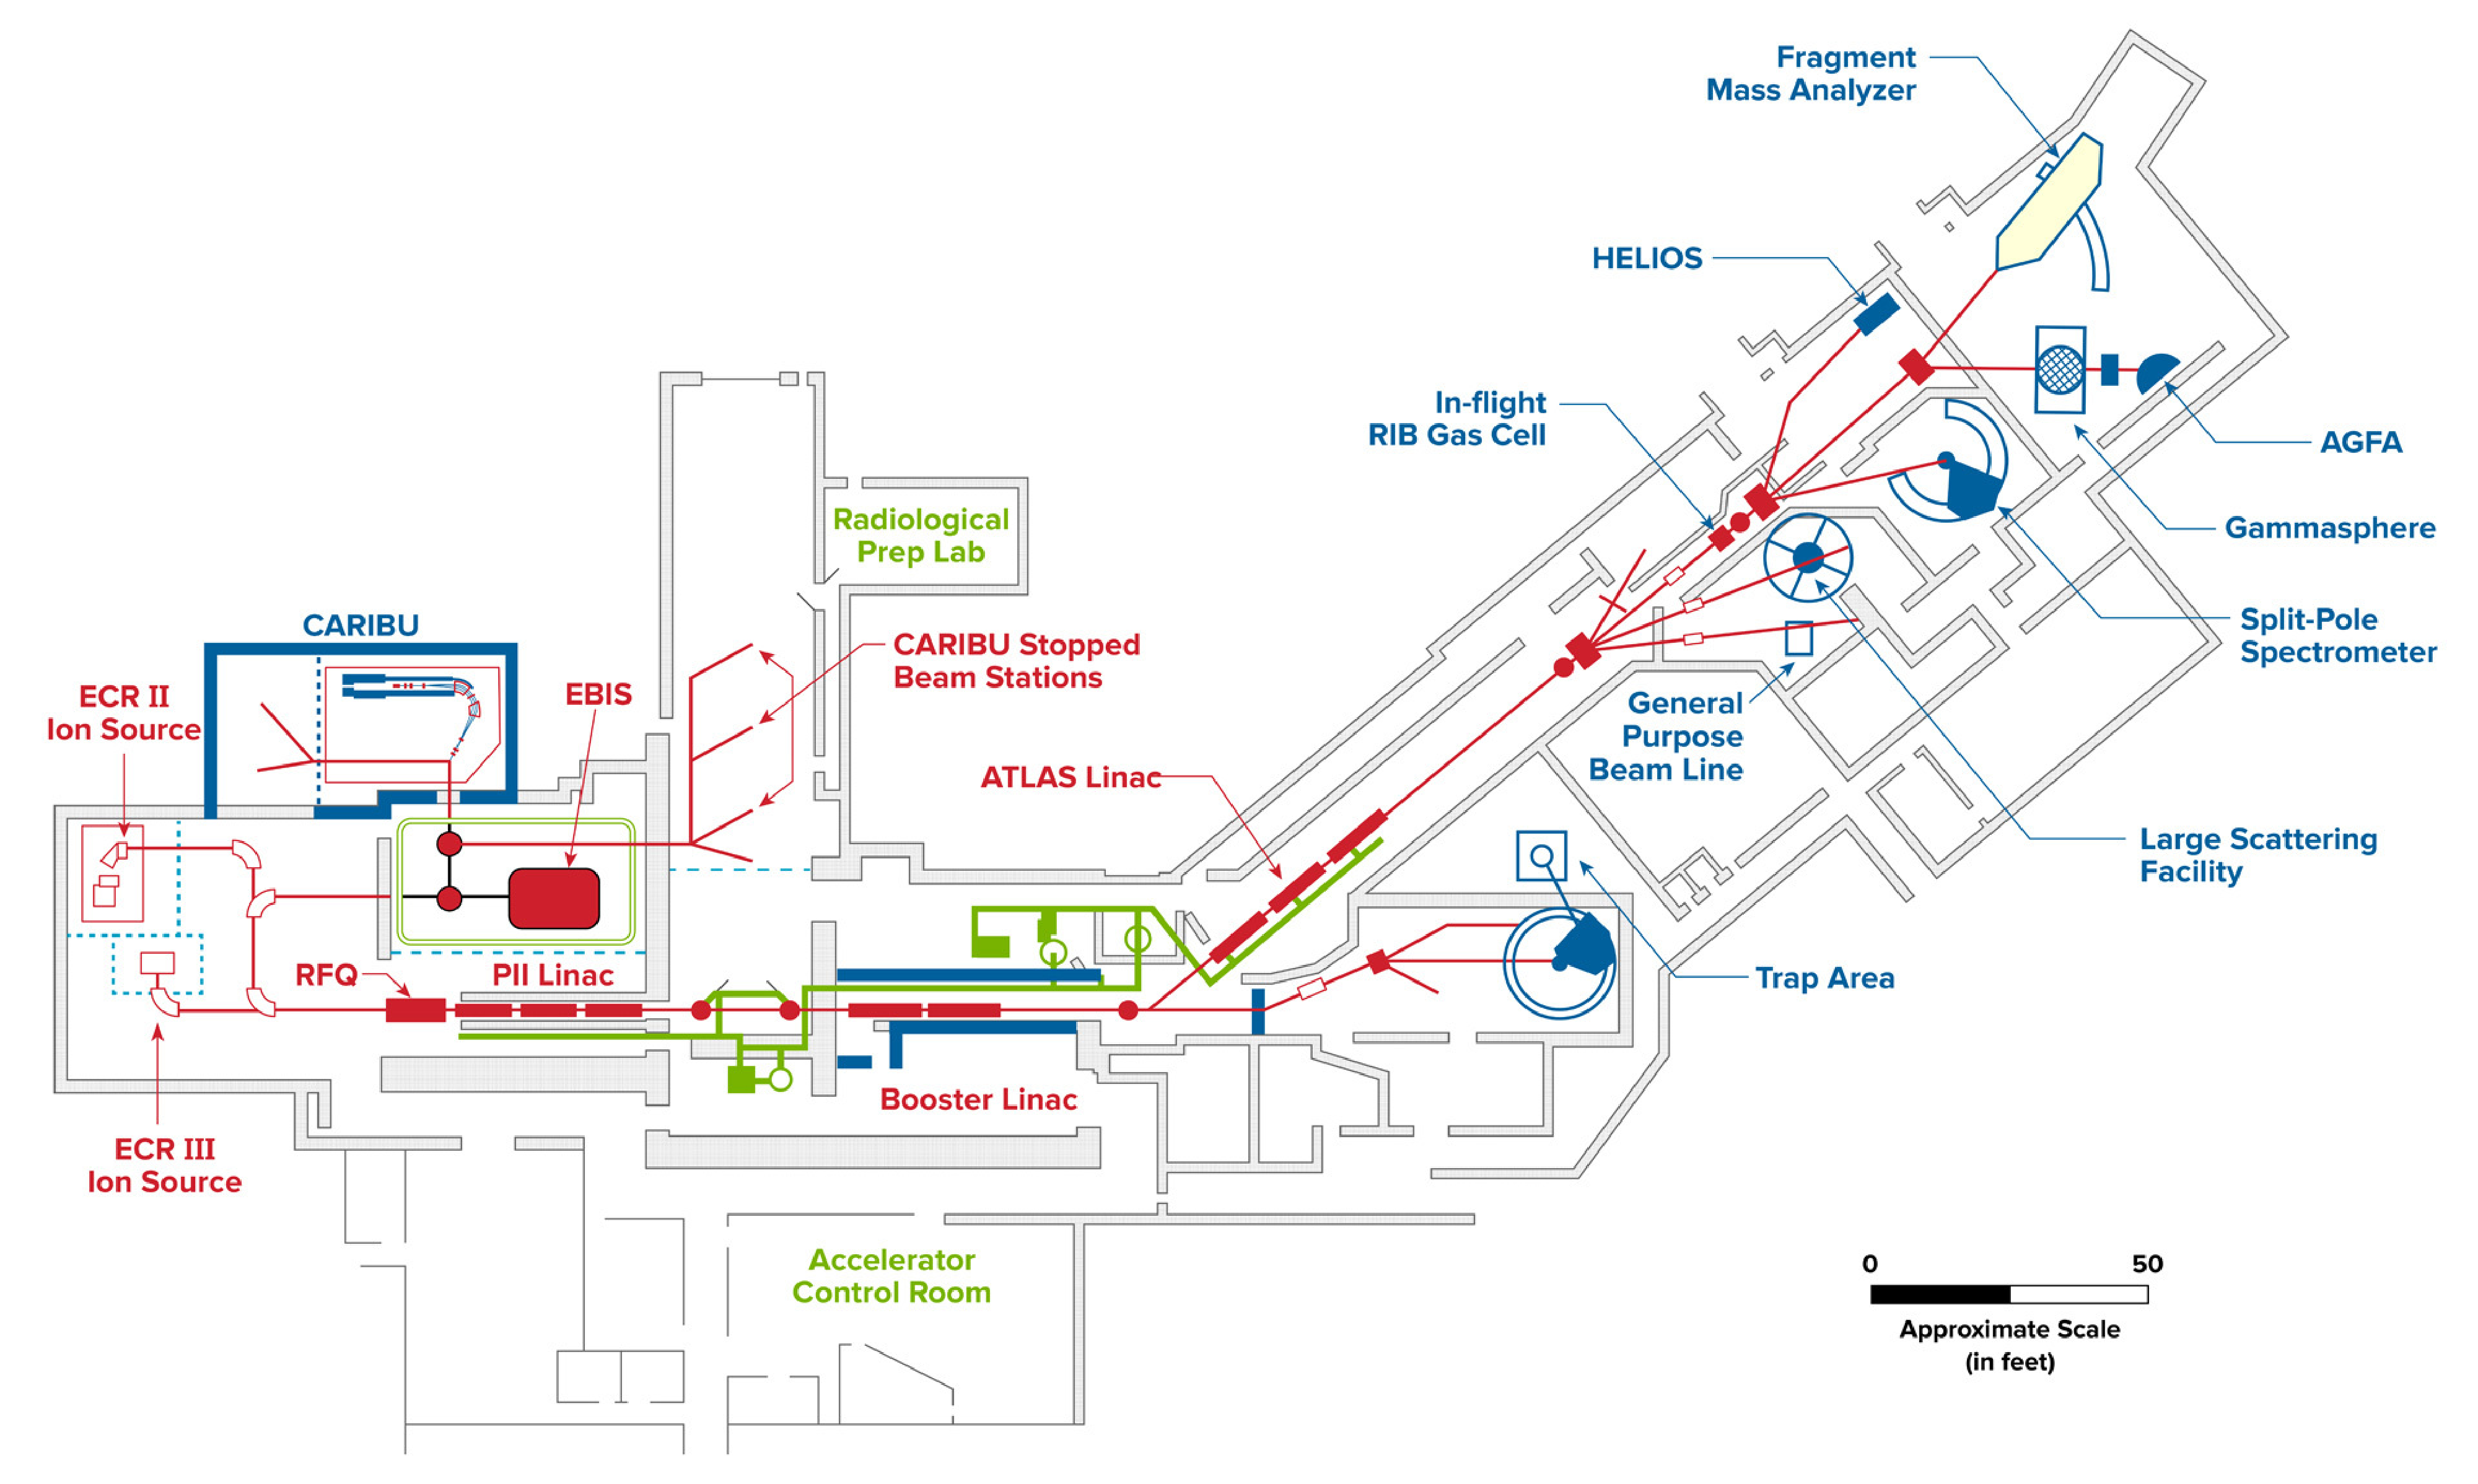
\includegraphics[width=\textwidth]{figures/floor-plan}
}% }}}
\frame{% whole pic for targets text {{{
	Рассмотрим элементы установки после мишеней.

	Анализатор фрагментов масс используется для разделения продуктов 
	реакции на интересующей мишени и непровзаимодействовавших ядер. Также 
	он используется в схеме совпадений при одновременной регистрации 
	фотонов и ядер. Также он используется и в обычном назначении -- для 
	определения отношения заряда к массе.

	HELIOS (Helical Orbit Spectrometer) это винтовой орбитальный 
	спектрометр или же спектрометр с винтовыми орбитами. Здесь мишень 
	располагается непосредственно внутри соленоида, который представляет 
	собой обычный магнит из МРТ. Мишень и детектор находятся на оси 
	соленоида, а продукты реакции загибаются и летят обратно к оси. 
	Детектор можно переставлять так, чтобы ловить продукты с определенной 
	энергией, зарядом и прочее. HELIOS используется для изучения реакции 
	передачи одного или нескольких нуклонов, кластеров, неупругого 
	рассеяния, используют в основном для нестабильных пучков.
}% }}}
\frame{% whole pic for targets text {{{
	AGFA -- argonne gas filled separator -- газовый сепаратор, 
	используется для изучения тяжелых и сверхтяжелых ядер. Например, для 
	поиска изомерных состояний в таких ядрах и изучения ядер вблизи 
	протонной радиоактивности, а также изучения тяжелых нейтроноизбыточных 
	ядер в глубоконеупругих реакциях.

	Gammasphere -- детектор фотонов, состоящий из 100 германиевых 
	детекторов.
}% }}}

\frame{% Program - Structure {{{
	\frametitle{Программа эксперимента. Структура ядер}

	\begin{itemize}\small
		\item Сравнение свойств ядер $A<20$ с вычислениями по модели оболочек.
		\item Исследование свойств нейтроноизбыточных ядер: изменения 
			в структуре оболочек, спаривание, новые коллективные возбуждения.
		\item Изучение воздействия слабой энергии связи на ядра вблизи 
			протонной радиоактивности: структура оболочек, деформация, 
			радиоактивность. Особое внимание области $N=Z$ при $50<A<100$, 
			а также вблизи $^{100}$Sn.
		\item Изучение ядер с зарядом $Z>100$ и проверка теорий, описывающих 
			сверхтяжелые ядра.
		\item Изучение свойств ядер при больших спинах и энергиях 
			возбуждения, включая взаимосвязь коллективных и одночастичных 
			степеней свободы, поиск новых коллективных мод и их спектральных 
			сигнатур по всей таблице, изучение зависимости плотности уровней 
			от углового момента и температуры.
	\end{itemize}
}% }}}
\frame{% Program - stars {{{
	\frametitle{Программа эксперимента. Нуклеосинтез в звездах}

	\begin{itemize}
		\item Измерение сечений реакций расширенного CNO-цикла.
		\item Измерение сечений $(\alpha, p)$ и $(p, \gamma)$ реакций на 
			пути $rp$-процесса.
		\item \what{Измерение сечений реакций между тяжелыми ионами при 
			энергиях, соответствующих горению в звездах.}
		\item Изучение реакций, ответственных за образование ядер 
			$p$-процесса.
		\item Изучение масс и свойств распадов ядер вблизи линии 
			$r$-процесса, в частности, вблизи $N=82, 126$ и в редкоземельном 
			пике.
	\end{itemize}
}% }}}
\frame{% Program - coloumb {{{
	\frametitle{Программа эксперимента. Динамика вблизи кулоновского барьера}

	\begin{itemize}
		\item Изучение подавления слияния при экстремальных подбарьерных 
			энергиях, особенно в системах, актуальных для ядерной астрофизики.
		\item Влияние ядерной структуры (деформация, структура оболочек, 
			диссипация и др.) на слияние, особенно для реакций, приводящих 
			к ядрам с $Z>100$.
		\item \what{Влияние избытка нейтронов на ядерные реакции вблизи 
			кулоновского барьера.}
	\end{itemize}
}% }}}
\frame{% Program - symmetries {{{
	\frametitle{Программа эксперимента. Проверка симметрий природы}

	\begin{itemize}
		\item {Поиски возможных расширений Стандартной модели путем 
			улучшения на порядок ограничений на скалярную, тензорную и правую 
			компоненты электрослабых взаимодействий.}
		\item {Проверка гипотезы сохранения векторного тока 
			и унитарности первого ряда матрицы Кабиббо-Кобаяши-Маскава путем 
			изучения бета-распадов.}
		\item \what{Изучение спектров антинейтрино в распадах продуктов 
			деления для определения природы видимой аномалии реакторных 
			нейтрино, наблюдавшейся в экспериментах по осцилляции нейтрино.}
	\end{itemize}
}% }}}
\frame{% Program - nucl applications {{{
	\frametitle{Программа эксперимента. Приложения ядерной физики}

	\begin{itemize}
		\item Использование ускорительной масс-спектрометрии для изучения 
			сечений захвата нейтронов различными изотопами, представляющими 
			интерес для реакторной физики и ядерной астрофизики.
		\item \what{Изучение свойств распада нейтроноизбыточных изотопов, 
			важных для точного моделирования динамики в новых циклах ядерного 
			топлива.}
		\item Использование бомбардировки тяжелыми ионами для изучения 
			повреждений материалов, рассматриваемых для передовых реакторов, 
			и модификации сверхпроводящих материалов.
		\item Разработка новых способов образования отдельных изотопов для 
			медицинских нужд.
	\end{itemize}
}% }}}

\frame{% Publications {{{
	\frametitle{Публикации -- названия говорят за себя}

	\begin{itemize}
		\item Proton decay of $^{108}$I and its significance for the 
			termination of the astrophysical $rp$-process.
			[Phys. Lett. B 792, 187 (2019)]

		\item Masses and $\beta$-Decay Spectroscopy of Neutron-Rich Odd-Odd 
			$^{160,162}$Eu Nuclei: Evidence for a Subshell Gap with Large 
			Deformation at N=98.
			[Phys. Rev. Lett. 120, 182502 (2018)]

		\item Direct Evidence of Octupole Deformation in Neutron-Rich 
			$^{144}$Ba.
			[Phys. Rev. Lett. 116, 112503 (2016)]

		\item Precision Mass Measurements of Neutron-Rich Neodymium and 
			Samarium Isotopes and Their Role in Understanding Rare-Earth Peak 
			Formation.
			[Phys. Rev. Lett. 120, 262702 (2018)]

		\item Shape Coexistence and the Role of Axial Asymmetry in $^{72}$Ge.
			[Phys. Lett. B 754, 254 (2016)]

		\item
			Modeling Multi-Nucleon Transfer in Symmetric Collisions of Massive 
			Nuclei.
			[Phys. Lett. B 771, 119 (2017)]

		\item Reaction rate for carbon burning in massive stars.
			[Phys. Rev. C 97, 012801 (2017)]

	\end{itemize}
}% }}}

\frame{% One publication {{{
	\frametitle{Proton decay of $^{108}$I and its significance for the termination of the astrophysical $rp$-process}

	\begin{columns}
		\column{.4\linewidth}{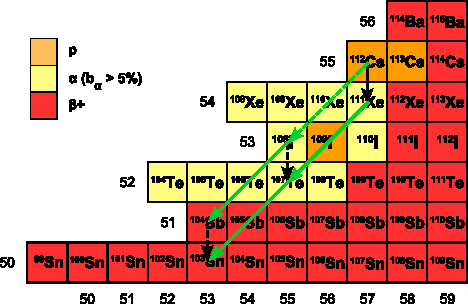
\includegraphics[width=\linewidth]{figures/nuclsynth}}
		\column{.6\linewidth}{
			$^{112}_{55}$Cs стабильнее $^{113}_{55}$Cs и, возможно, 
			$^{104}$Sb~стабильнее ожидаемого. Тогда именно через него идет 
			путь $rp$-процесса.

			Для нахождения $Q_p(^{104}\text{Sb})$ ищется $Q_p(^{108}\text{I})$.
		}
	\end{columns}

	$$ ^{58}\text{Ni} + ^{54}\text{Fe} \to ^{108}\text{I} + p + 3n $$

	\begin{itemize}

		\item Выделялись ионы c $A = {108}$ и зарядом ${+26,+27}$.

		\item Рассматривались цепи событий попадание-распад 
			и попадание-распад-распад в одном и том же пикселе кремниевого 
			детектора.
	\end{itemize}
}% }}}
\frame{% One publication {{{
	\frametitle{Proton decay of $^{108}$I and its significance for the termination of the astrophysical $rp$-process}
	\centering
	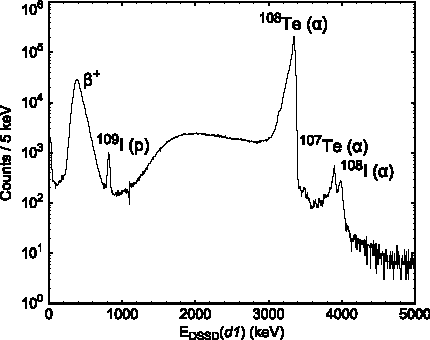
\includegraphics[width=.7\linewidth]{figures/i-108-energy}

	\small Все распады без каких-либо отборов.
}% }}}
\frame{% One publication {{{
	\frametitle{Proton decay of $^{108}$I and its significance for the termination of the astrophysical $rp$-process}
	\centering
	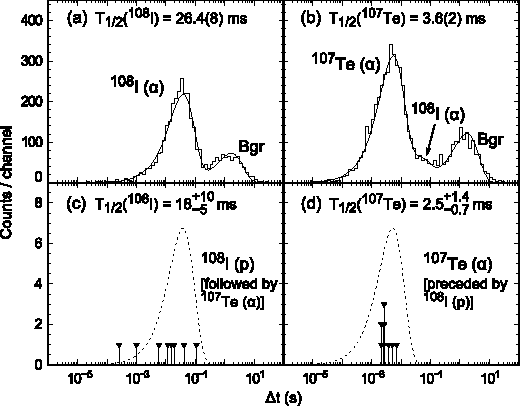
\includegraphics[width=.7\linewidth]{figures/i-108-decays}

	\small Все распады и парциальные распады по определенным каналам.
}% }}}
\frame{% One publication {{{
	\frametitle{Proton decay of $^{108}$I and its significance for the termination of the astrophysical $rp$-process}
	\centering
	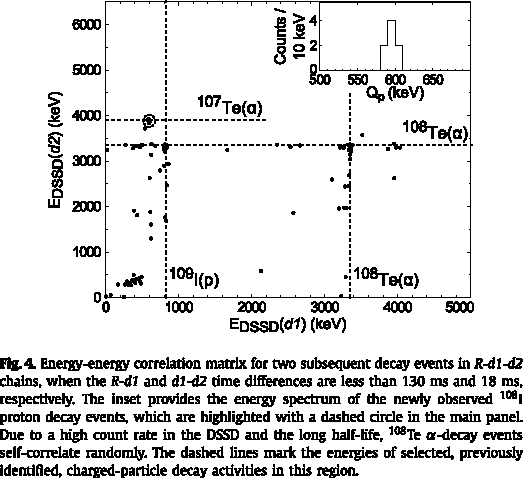
\includegraphics[width=.6\linewidth]{figures/i-108-2d-chart}
}% }}}
\frame{% One publication {{{
	% Для начала рассмотрим сам йод 108. В сферической модели оболочек 
	% квазиклассическое приближение дает парциальное время жизни 150 мс 
	% или 70 с для вылета из d и g состояния соответственно. Полученное 
	% в работе значение 5 с находится ровно между этими, то есть 
	% с уверенностью можно сказать лишь что состояния сильно смешиваются. 
	% Однако можно предположить, что деформация йода 108 примерно такая, 
	% как у 109, а одиночные протон и нейтрон располагаются на смесях 1/2+ 
	% и 3/2+ по схеме Нильсона. Учитывая ожидаемый спин Te 107, 
	% получается, что преобладать должен l=2 протон.
	%
	% Теперь касательно сурьмы 104.
	\frametitle{Proton decay of $^{108}$I and its significance for the termination of the astrophysical $rp$-process}
	\centering
	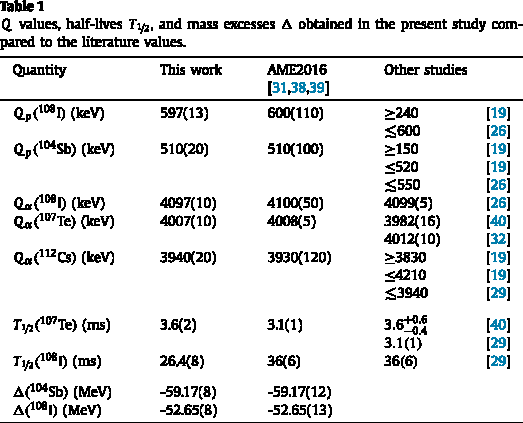
\includegraphics[width=.7\linewidth]{figures/i-108-table}
}% }}}
\frame{% One publication text {{{
	\frametitle{Proton decay of $^{108}$I and its significance for the 
	termination of the astrophysical $rp$-process}

	Для начала рассмотрим сам йод 108. В сферической модели оболочек 
	квазиклассическое приближение дает парциальное время жизни 150 мс и 70 
	с для вылета из $d$ и $g$ состояния, соответственно. Полученное 
	в работе значение 5 с находится ровно между этими, то есть 
	с уверенностью можно сказать лишь что состояния сильно смешиваются. 
	Однако можно предположить, что деформация йода 108 примерно такая, как 
	у 109, а одиночные протон и нейтрон располагаются на смесях 
	$\frac{1}{2}^+$ и $\frac{3}{2}^+$ по схеме Нильсона. Учитывая 
	ожидаемый спин Te 107, получается, что преобладать должен $l=2$ 
	протон.

	\hrulefill
	\small

	Эта статья не может похвастаться прорывным результатом, но, мне 
	кажется, она все равно хорошо демонстрирует производимую на ATLAS 
	работу.
}% }}}

\frame{% Future {{{
	\frametitle{Будущее ATLAS в ANL}

	\begin{itemize}
		\item Использование CARIBU для получения и изучения 
			нейтроноизбыточных ядер при низких энергиях.

		\item Модернизация сверхпроводников и увеличение максимальной 
			энергии для получения новых радиоактивных изотопов на лету 
			в реакциях с большой передачей импульса.

		\item Переход на сверхпроводники в источниках ионов для увеличения 
			интенсивности пучков стабильных ядер и ядер, образующихся на лету.

		\item Создание генератора нейтронов и замена калифорния в CARIBU 
			на~тонкую фольгу из актинидов, которые будут испытывать 
			вынужденное деление под действием нейтронов из генератора.

		\item Внедрить стабильные пучки в интервалы между пучками от CARIBU, 
			что позволит увеличить время работы установки на 35--50\%.
	\end{itemize}
}% }}}

\end{document}

===============================================
===============================================
===============================================

ATLAS	ANL (USA)

доклад + реферат
1. Технические характеристики (диапазоны ядер, энергии, светимости и т.д.)
2. Особенности получения, ускорения, детектирования
3. Программа экспериментов
4. Основные результаты 
5. Проекты дальнейшего развития
6. Как минимум разобрать и показать одну конкретную статью с результатами от коллаборации
